%% This is file `elsarticle-template-1-num.tex',
%%
%% Copyright 2009 Elsevier Ltd
%%
%% This file is part of the 'Elsarticle Bundle'.
%% ---------------------------------------------
%%
%% It may be distributed under the conditions of the LaTeX Project Public
%% License, either version 1.2 of this license or (at your option) any
%% later version.  The latest version of this license is in
%%    http://www.latex-project.org/lppl.txt
%% and version 1.2 or later is part of all distributions of LaTeX
%% version 1999/12/01 or later.
%%
%% Template article for Elsevier's document class `elsarticle'
%% with numbered style bibliographic references
%%
%% $Id: elsarticle-template-1-num.tex 149 2009-10-08 05:01:15Z rishi $
%% $URL: http://lenova.river-valley.com/svn/elsbst/trunk/elsarticle-template-1-num.tex $
%%
\documentclass[preprint,12pt]{elsarticle}

%% Use the option review to obtain double line spacing
%% \documentclass[preprint,review,12pt]{elsarticle}

%% Use the options 1p,twocolumn; 3p; 3p,twocolumn; 5p; or 5p,twocolumn
%% for a journal layout:
%% \documentclass[final,1p,times]{elsarticle}
%% \documentclass[final,1p,times,twocolumn]{elsarticle}
%% \documentclass[final,3p,times]{elsarticle}
%% \documentclass[final,3p,times,twocolumn]{elsarticle}
%% \documentclass[final,5p,times]{elsarticle}
%% \documentclass[final,5p,times,twocolumn]{elsarticle}


\biboptions{comma} % Multiple refs will be separated with semicolon

\journal{Physical Review C}

% PFS Custom commands
% \input{latex_defs}
% % My (and Erik's) custom functions
% % Don't forget to use
\usepackage{xspace}

% References and citations
\newcommand{\fig}[1]     {Fig.~\ref{#1}}
\newcommand{\figfirst}[1]  {Figure~\ref{#1}}
\newcommand{\tab}[1]     {Table~\ref{#1}}
\newcommand{\chapref}[1] {Chap.~\ref{#1}}
\newcommand{\secref}[1]  {Sec.~\ref{#1}}
\newcommand{\eqnref}[1]  {Eq.~\eqref{#1}}
\newcommand{\refref}[1]  {Ref.~\cite{#1}}
\newcommand{\refrefs}[1]  {Refs.~\cite{#1}}
\newcommand{\appref}[1]  {App.~\ref{#1}}
\newcommand{\etal}       {\textit{et~al.}\xspace}

\newcommand{\rephrase}[1]     {\color{violet}[Rephrase: #1]\color{black}\xspace}
\newcommand{\directcopy}[2]   {\color{violet}[Copied Directly from #1:  #2]\color{black}\xspace}

% Custom phrases
\newcommand{\MPPost}          {\texttt{MPPost}\xspace}
\newcommand{\mcnpxpolimi}     {\texttt{MCNPX-PoliMi}\xspace}
\newcommand{\cgmf}            {\texttt{CGMF}\xspace}
\newcommand{\freya}           {\texttt{FREYA}\xspace}
\newcommand{\polimi}          {\texttt{POLIMI}\xspace}
\newcommand{\polimiipol}      {\texttt{MCNPX-POLIMI IPOL(1)=1}\xspace}
\newcommand{\coloronline}     {(Color online)\xspace}

% For FNPC paper
\newcommand{\Dt}{\ensuremath{\Delta t}\xspace}
\newcommand{\Dti}{\ensuremath{\Delta t_i}\xspace}
\newcommand{\Dto}{\ensuremath{\Delta t_1}\xspace}
\newcommand{\Dtt}{\ensuremath{\Delta t_2}\xspace}
\newcommand{\Dtct}{\ensuremath{\Delta t_{CT}}\xspace}
\newcommand{\Dtot}{\ensuremath{\Delta t_{1\rightarrow2}}\xspace}
\newcommand{\Dtto}{\ensuremath{\Delta t_{2\rightarrow1}}\xspace}


\newcommand{\Eo}{\ensuremath{E_1}\xspace}
\newcommand{\Et}{\ensuremath{E_2}\xspace}
\newcommand{\Emin}{\ensuremath{E_{\textrm{min}}}\xspace}
\newcommand{\Ei}{\ensuremath{E_i}\xspace}
\newcommand{\Ej}{\ensuremath{E_j}\xspace}
\newcommand{\Eave}{\ensuremath{\overline{E_n}}\xspace}
\newcommand{\Ejave}{\ensuremath{\overline{E_j}}\xspace}

\newcommand{\Cpos}{\ensuremath{C_{pos}}\xspace}
\newcommand{\Cneg}{\ensuremath{C_{neg}}\xspace}
\newcommand{\Cnet}{\ensuremath{C_{net}}\xspace}


\newcommand{\Si}            {\ensuremath{S_{i}}\xspace}
\newcommand{\Sj}            {\ensuremath{S_{j}}\xspace}
\newcommand{\Dij}            {\ensuremath{D_{ij}}\xspace}
\newcommand{\W}              {\ensuremath{W}\xspace}
\newcommand{\Wij}            {\ensuremath{W_{ij}}\xspace}
\newcommand{\Wtheta}         {\ensuremath{\overline{W}(\theta)}\xspace}
\newcommand{\Wth}[1]         {\ensuremath{\overline{W}(\degrees{#1})}\xspace}
\newcommand{\Asym}           {\ensuremath{A_{\rm{sym}}}\xspace}

% % Units typeset in roman
\newcommand{\genunit}[2]{\ensuremath{#1~\text{#2}}\xspace}
\newcommand{\meters}[1] {\genunit{#1}{m}}
\newcommand{\cm}[1]     {\genunit{#1}{cm}}
% \newcommand{\keV}[1]    {\genunit{#1}{keV}}
% \newcommand{\keVee}[1]  {\genunit{#1}{keVee}}
\newcommand{\MeV}[1]    {\genunit{#1}{MeV}}
% \newcommand{\MeVee}[1]  {\genunit{#1}{MeVee}}
% \newcommand{\TeV}[1]    {\genunit{#1}{TeV}}
% \newcommand{\GeV}[1]    {\genunit{#1}{GeV}}
% \newcommand{\pb}[1]     {\genunit{#1}{pb}}
% \newcommand{\inch}[1]   {\genunit{#1}{in}}
% \newcommand{\hours}[1]  {\genunit{#1}{h}}
% \newcommand{\minutes}[1]{\genunit{#1}{min}}
\newcommand{\ns}[1]{\genunit{#1}{ns}}

% % these units have some funny business like exponents, c, etc.
% \newcommand{\uCi}[1]    {\ensuremath{#1~\mu\mathrm{Ci}}\xspace}
% \newcommand{\cmsq}[1]   {\ensuremath{#1~\mathrm{cm}^{2}}\xspace}
% \newcommand{\cmcub}[1]  {\ensuremath{#1~\mathrm{cm}^{3}}\xspace}
% \newcommand{\MeVcc}[1]  {\ensuremath{#1~\mathrm{MeV}/c^{2}}}
% \newcommand{\GeVc}[1]   {\ensuremath{#1~\mathrm{GeV}/c}}
% \newcommand{\GeVcc}[1]  {\ensuremath{#1~\mathrm{GeV}/c^{2}}}
% \newcommand{\invpb}[1]  {\ensuremath{#1~\mathrm{pb}^{-1}}}
% \newcommand{\invfb}[1]  {\ensuremath{#1~\mathrm{fb}^{-1}}}
\newcommand{\degrees}[1]{\ensuremath{#1^{\mathrm{o}}}\xspace}
% \newcommand{\sigcunit}[1]{\ensuremath{#1~\mathrm{\sigma_{c}}}\xspace}
% \newcommand{\sigunit}[1]{\ensuremath{#1~\mathrm{\sigma}}\xspace}
% \newcommand{\us}[1]     {\ensuremath{#1~\mu\mathrm{s}}\xspace}
% \newcommand{\um}[1]     {\ensuremath{#1~\mu\mathrm{m}}\xspace}
% \newcommand{\npercmsqsec}[1]{\ensuremath{#1~\mathrm{n}/\mathrm{cm}^{2}/\mathrm{s}}\xspace}
% \newcommand{\gpercmcub}[1]{\ensuremath{#1~\mathrm{g}/\mathrm{cm}^{3}}\xspace}

% % Isotopes
\newcommand{\Csots}{\ensuremath{^{137}\text{Cs}}\xspace}
\newcommand{\Natt} {\ensuremath{^{22}\text{Na}}\xspace}
\newcommand{\Cftft}{\ensuremath{^{252}\text{Cf}}\xspace}
\newcommand{\Cftfo}{\ensuremath{^{250}\text{Cf}}\xspace}
\newcommand{\Cmtfe}{\ensuremath{^{248}\text{Cm}}\xspace}
\newcommand{\Putf}{\ensuremath{^{240}\text{Pu}}\xspace}


% %%%%%%%%%%%%%%% Packages %%%%%%%%%%%%%%%%%%%%%%%%%%%%%%%%%%%%%%%%%%%%%%%

\usepackage[margin=.80in]{geometry}
\usepackage[doublespacing]{setspace}
% %% From ucbthesis
% %\usepackage[sorting=none]{biblatex}						% Number citations based on when they are introduced
% %\usepackage{url}                                        % For misc entries that contain \url{} 
%\usepackage[doi=false,isbn=false,url=false]{biblatex}   % Leave DOI, ISBN, and URL out of bibliography
\usepackage{xcolor}                                     % Extra font colors
% \usepackage[usenames, dvipsnames]{color}
\usepackage{amssymb}                                    % Math symbols
\usepackage{amsmath,amsthm}
% %\usepackage{amsthm}                                     % The amsthm package provides extended theorem environments
% \usepackage{epstopdf}                                   % Use .eps images
% \usepackage{subfigure}
\usepackage[caption=false,font=footnotesize,subrefformat=parens,labelformat=parens]{subfig}    % Use subfigures
\usepackage{graphicx}                           % The graphicx package provides the includegraphics command.
% \usepackage{float}                                    % Not needed with `caption`
% \usepackage{placeins}
% %\usepackage{subcaption}
% %\usepackage{caption}
% \usepackage{multirow}                                   
% \usepackage{etoolbox}                                   % Hack references
\usepackage[hidelinks]{hyperref}                        % Links in text
\hypersetup{                    
	colorlinks,
	citecolor=black,
	filecolor=black,
	linkcolor=black,
	urlcolor=black
}
% \usepackage[capitalise]{cleveref}						  % Clever references
% {equation}{Eq.~#2#1#3}						  % Don't use () in Eqn.
% \usepackage{verbatim}                                   % Verbatim
% \usepackage[makeroom]{cancel}                           % Cross out canceled terms in equations
% \usepackage[utf8]{inputenc}                             % Try to fix problems with characters in bib file
\usepackage{listings}                                   % Box around code
% \usepackage[framed]{matlab-prettifier}                  % Display matlab code
% \usepackage{enumitem}									  % Additional enumerate/itemize options
% \usepackage{easy}             						  % easy table
% %\usepackage[none]{hyphenat}							  % Remove all hyphenating between lines
\usepackage{lineno}										  % Add line numbers.
\linenumbers 
% Start: \begin{linenumbers}
%                                                               % End:   \end{linenumbers}
%                                                               % On for whole: \linenumbers (after \end{frontmatter})
% %%%%%%%%%%%%%%%%%%%%%%%%%%%%%%%%%%%%%%%%%%%%%%%%%%%%%%%%%%%%%%%%%%%%%%%%%%



% Turn comments on or off
\newif\ifshowcomments
\showcommentsfalse


\begin{document}


%%%%%%%%%%%%%%%%%%%%%%%%%%%%% FRONT MATTER %%%%%%%%%%%%%%%%%%%%%%%%%%%%%%%
\begin{frontmatter}

\title{High resolution measurement of tagged two-neutron energy and angle correlations in \Cftft(sf)}

%% use the tnoteref command within \title for footnotes;
%% use the tnotetext command for the associated footnote;
%% use the fnref command within \author or \address for footnotes;
%% use the fntext command for the associated footnote;
%% use the corref command within \author for corresponding author footnotes;
%% use the cortext command for the associated footnote;
%% use the ead command for the email address,
%% and the form \ead[url] for the home page:
%%
%% \title{Title\tnoteref{label1}}
%% \tnotetext[label1]{}
%% \author{Name\corref{cor1}\fnref{label2}}
%% \ead{email address}
%% \ead[url]{home page}
%% \fntext[label2]{}
%% \cortext[cor1]{}
%% \address{Address\fnref{label3}}
%% \fntext[label3]{}


%% use optional labels to link authors explicitly to addresses:
%% \author[label1,label2]{<author name>}
%% \address[label1]{<address>}
%% \address[label2]{<address>}

%%%%%%%%%%%%%%%%%%%%%%%%%%%% AUTHOR INFO %%%%%%%%%%%%%%%%%%%%%%%%%%%%%%

\author[umich]{P.~F.~Schuster\corref{cor1}}
\ead{pfschus@umich.edu}
\author[umich]{M.~J.~Marcath}
\author[umich]{S.~Marin}
\author[umich]{S.~D.~Clarke}
\author[lanl]{M.~Devlin}
\author[lanl]{R.~C.~Haight}
\author[llnl,ucdavis]{R.~Vogt}
\author[lanl]{P.~Talou}
\author[lanl]{I.~Stetcu}
\author[lanl]{T.~Kawano}
\author[lbnl]{J.~Randrup}
\author[umich]{S.~A.~Pozzi}

\cortext[cor1]{Corresponding author}

\address[umich]{Department of Nuclear Engineering and Radiological Sciences, University of Michigan, Ann Arbor, MI 48109, USA}
\address[lanl]{T-2, Los Alamos National Laboratory, Los Alamos, New Mexico, 87545, USA}
\address[llnl]{Nuclear and Chemical Sciences Division, Lawrence Livermore National Laboratory, Livermore, CA 94551, USA}
\address[ucdavis]{Department of Physics, University of California, Davis, California 95616, USA}
\address[lbnl]{Nuclear Science Division, Lawrence Berkeley National Laboratory, Berkeley, CA, USA}

%%%%%%%%%%%%%%%%%%%%%%%%%%%%%%%% ABSTRACT %%%%%%%%%%%%%%%%%%%%%%%%%%%%%

\begin{abstract}
%% Text of abstract

\noindent \textbf{Background:} Spontaneous fission events emit prompt neutrons correlated with one another in emission angle and energy. Measurements of these correlations can shed light on the partitioning of the excitation energy between the fragments, even if they are not directly measured.

\noindent \textbf{Purpose:} We explore the relationship in energy and angle between correlated prompt neutrons emitted from \Cftft spontaneous fission.

\noindent \textbf{Methods:} Measurements with the Chi-Nu array provide experimental data for coincident neutrons tagged with a fission chamber signal with \degrees{10} angular resolution and \ns{1} timing resolution for time-of-flight energy calculations. The experimental results are compared to simulations produced by the fission event generators \cgmf, \freya, and \polimiipol.

\noindent \textbf{Results:} We find that the measurements and the simulations all exhibit anisotropic neutron emission, although differences between fission event generators are evident.

\noindent \textbf{Conclusions:} This work shows that the dependence of detected neutron energy on the energy of another neutron detected in coincidence, although weak, is non-negligible, indicating that there may be correlations in energy between two neutrons emitted in the same fission event.






\end{abstract}

\begin{keyword}
Fission \sep Neutron \sep Correlation

\end{keyword}

\end{frontmatter}

\section{Introduction}

In a fission event, prompt neutron emission occurs on a time scale shorter than that of gamma-ray emission~\cite{Fraser1952a,Skarsvag1970}. The emitted neutrons are correlated with one another in their emission angle and energy~\cite{Bowman1962,Larsen2014}. Measurements of these correlations can shed light on the partitioning of the excitation energy between the fragments, even if they are not directly measured. The commonly used \mcnpxpolimi Monte Carlo code treats such correlations using data-based evaluations~\cite{Pozzi2012}. The new, physics-based fission models \cgmf~\cite{Talou2013,Talou2014,Talou2016} and \freya~\cite{Randrup2009,Vogt2011,Vogt2013,Vogt2014,Randrup2014,Vogt2017,Verbeke2018} generate complete events and can thus produce correlations between emitted particles on an event-by-event basis. These codes require high fidelity experimental data for validating their models. In this paper, we describe our \Cftft spontaneous fission data, correlated in neutron energy and two-neutron angular separation, and compare the measured correlations to those simulated with the fission models \mcnpxpolimi, \cgmf, and \freya, each using \mcnpxpolimi for radiation transport and \MPPost~\cite{Miller2012} for detector response.

Numerous detector systems exist or are in development for nuclear nonproliferation, safeguards, and arms control applications that would benefit from a better understanding of the correlations in prompt fission neutron emission. One such example is the fast neutron multiplicity counter, a nuclear safeguards instrument that is used for nondestructive assay of special nuclear material~\cite{Frame2007,DiFulvio2017}. 
Similarly, applications have been proposed for exploiting the correlations that exist between neutrons emitted from the same fission event in multiplying materials where fission chains are present~\cite{Mueller2016,Holewa2013}. 
Accurate physics models are important in the development of these systems and methods.

This paper presents measurements and simulations of correlated neutrons from \Cftft spontaneous fission to confirm and extend previously reported results. Measurements were made with 42 detectors of the Chi-Nu detector array at the Los Alamos Neutron Science Center (LANSCE) at Los Alamos National Laboratory (LANL)~\cite{Perdue2014,MarcathThesis2018}. The Chi-Nu array covers a large solid angle with detectors approximately \meters{1} from the source, thereby providing high efficiency and excellent timing resolution for time-of-flight energy calculations. Additionally, the \Cftft source was embedded in a fission chamber, providing good time resolution for the fission event signal. Double coincident neutron events, in which two neutrons are detected in coincidence with a fission chamber trigger, were identified as ``bicorrelation'' events, as explained in \secref{sec:bicorr_events}. 
The measurement offers improved angle resolution, excellent timing resolution, and enhanced background suppression compared to previous work~\cite{Larsen2014,Verbeke2018b}. A previous paper by the authors investigated correlations between the prompt neutron and photon multiplicities~\cite{Marcath2018}. This work includes the first comparison of correlated neutron energy characteristics for \Cftft spontaneous fission, including a new observable: the average energy of neutrons detected in coincidence with emitted neutrons at a given energy as a function of the angle between them.


\section{Experimental, Simulation, and Analysis Methods}

\subsection{Measurement Setup and Methods}

In this work, we employ the data taken with the Chi-Nu detector array, illustrated in \fig{fig:chi_nu_diagram}, at the LANL LANSCE facility in 2015, using a \Cftft spontaneous fission source, for our bicorrelation analysis. Because the experimental setup for this analysis was described in detail in \refrefs{Marcath2018,MarcathThesis2018}, we only briefly summarize the parts of the setup relevant for this analysis here. 
%An illustration of the detector array is shown in~\cref{fig:chi_nu_diagram} and 
The Chi-Nu array consists of 54 EJ309 liquid scintillator detectors mounted at \degrees{15} intervals along six arcs to form a hemispherical distribution of detectors. Each detector is cylindrical, \cm{17.78} in diameter and \cm{5.08} thick, coupled to a \cm{12.7} diameter photomultiplier tube (Hamamatsu R4144). Each detector subtends approximately a \degrees{10} angle from the source.
Limitations in the acquisition system constrained these measurements to using only 42 detectors, making for 861 pairs of detectors at angles from \degrees{15} to \degrees{180}. The large number of detector pairs produces a wide range of angles, allowing for discretization in \degrees{10} bins, as shown in \fig{fig:det_df}, which is improved compared to previous work with only \degrees{30} or \degrees{90} resolution~\cite{Larsen2014,Mueller2016}. Each \degrees{10} bin contains multiple detector pairs. The standard deviation of detector pair angles within each bin is represented as the bar color in \fig{fig:det_df}. Observable quantities are averaged across all pairs within a bin to reduce statistical error per bin. 

A \Cftft(sf) source was embedded in a fission chamber, with characteristics detailed in~\refref{Marcath2018}. To summarize, the Californium source was deposited over a hemispherical chamber. One or two fragments from a fission event may produce a pulse by escaping the surface and depositing energy through ionization. This trigger signal was used as the fission time $t_0$ for each detected event, as explained in \secref{sec:bicorr_events}. The fission chamber has a fixed threshold to exclude $\alpha$-particle interactions~\cite{Oberer2000}. The source was fabricated in 2010 and the measurements reported here were performed in 2015. The \Cftft spontaneous fission count rate was $2.98\times10^5$ spontaneous fissions per second, with negligible contributions from spontaneous fission of \Cftfo and \Cmtfe.  The source was placed at the focal point of the hemispherical array so that the detectors were approximately \meters{1} from the source. Over the duration of the measurement, $2.2\times10^9$ fission events occurred, resulting in $1.42\times10^9$ fission chamber triggers. 

The use of the fission chamber makes this measurement unique compared to similar measurements made in the past because it provides a reference time for when a fission event occurs. Thus the neutron time-of-flight may be directly calculated for each detected neutron whereas previous work was limited to calculating the difference between the detection times of correlated particles~\cite{Larsen2014}.  



\begin{figure}[h]
	\centering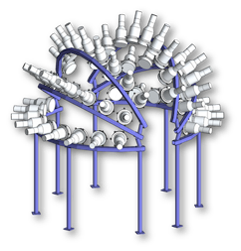
\includegraphics[scale=1]{setup.png}
	\caption{Diagram of the Chi-Nu detector array of 54 detectors. For this work, only 42 detectors were used.}
	\label{fig:chi_nu_diagram}
\end{figure}

\begin{figure}[!t]
	\centering
	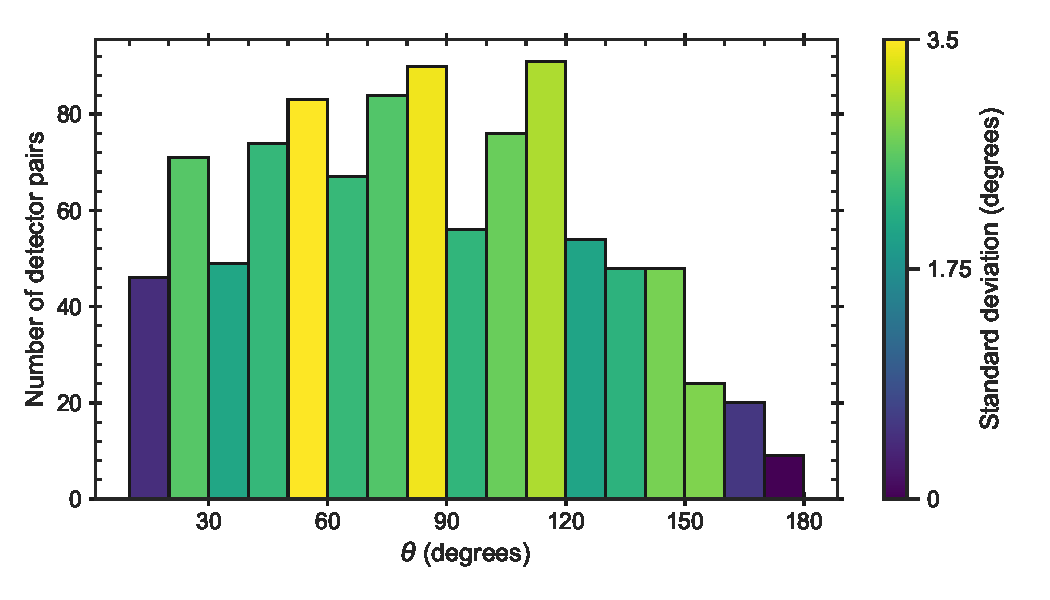
\includegraphics[trim={0cm 0cm 0cm 0cm},clip,width=.75\linewidth]{det_df_histogram.pdf}%	
	
	\caption{Visualization of detector pair angle distribution, discretized to \degrees{10} bins. The height of each bar shows the number of detector pairs in each bin. The color of each bar provides the standard deviation of detector pair angles within each bin. The bin containing $(\degrees{170},\degrees{180}]$, for example, is darkest because all pairs within that bin are at exactly \degrees{180}, producing the lowest standard deviation of \degrees{0}.}
	\label{fig:det_df}
\end{figure}

Full waveforms were recorded with three CAEN V1730 digitizers with 500 MHz sampling and 14-bit amplitude resolution over a 2 V range and post-processed in digital form. Standard digital pulse processing was implemented, as detailed in~\refref{Marcath2018}. Particle types were classified using charge-integration $n$-$\gamma$ pulse shape discrimination (PSD)~\cite{Polack2015}, which was performed offline and optimized uniquely for each detector. 
A quadratic PSD line was used to discriminate between the neutrons and photons with misclassification of low light output events estimated to be approximately 1\% of all measured events. 

The measurement had a pulse height threshold of 100 keVee (``electron-equivalent'' keV) light output, corresponding to approximately \MeV{0.8} neutron energy deposited. This threshold was selected to minimize misclassification of photons as neutrons in the measurement, which mostly occurs below this threshold. An upper voltage limit reduced the experimental sensitivity to neutrons with energy depositions above \MeV{8.1}. This work focuses on events where both detected neutrons have energies in the range \MeV{1} to \MeV{4} due to reduced statistics at higher energies. 

\subsection{Simulation Techniques}

The experimental setup was simulated using \mcnpxpolimi, which models the laboratory geometry and performs the particle transport. The system was modeled in great detail, including the Chi-Nu structure, concrete floor, and fission chamber. Waveform processing and particle-type classification is assumed to be perfect in the simulation so that all events are identified as the correct particle type. A light output threshold of 100 keVee was used to match that of the experimental data. 

In order to study different fission models, \cgmf, \freya, and the built-in PoliMi source \texttt{IPOL(1)=1}, referred to as \polimi, were used in \mcnpxpolimi. The similarities and differences between \freya and \cgmf are discussed in a recent article~\cite{Talou2018}, as well as some information about \polimi. These models produced list-mode data including initial energy, initial direction, and particle type for each particle generated in an individual fission event, which was passed to \mcnpxpolimi for transport. Following transport, \mcnpxpolimi produced a file with event-by-event information on interactions in detector cells. Detector response was calculated with \MPPost post-processing software~\cite{Miller2012}, which handles the nonlinear light output of organic scintillators.

\polimi and \freya simulated $10^9$ fission events, while $1.92\times10^8$ \cgmf events were employed, resampled with new, randomly sampled, fission fragment directions from a subset of $1.92\times10^6$ events. \tab{tab:counts} shows these values and the number of detected bicorrelation events in all four datasets.

\begin{table}[ht]
	\centering
	\caption{Experimentally detected and generated fission events resulting in the given total and per fission bicorrelation counts.}
	\label{tab:counts}
	\begin{tabular}{l|c|c|c}
		&number fissions& bicorrelation counts & bicorrelation counts per fission \\
		\hline
		Experiment   & $1.42\times10^9$ & $(3.941\pm0.002)\times10^6$ & $(2.771\pm0.002) \times10^{-3}$ \\
		\cgmf         & $1.92\times10^8$ & $(0.737\pm0.085)\times10^6$ & $(1.786\pm0.004) \times10^{-3}$\\
		\freya        & $1.00\times10^9$ & $(2.978\pm0.002)\times10^6$ & $(2.978\pm0.002) \times10^{-3}$\\
		\polimi       & $1.00\times10^9$ & $(3.409\pm0.002)\times10^6$ & $(3.409\pm0.002) \times10^{-3}$       
	\end{tabular}
\end{table}

\subsection{Identifying Bicorrelation Events}\label{sec:bicorr_events}

This paper studies the relationship between pairs of detected neutrons that are emitted from the same fission event, as illustrated in~\fig{fig:sketch}. The interaction times of two neutrons, $t_1$ and $t_2$, were each correlated with the corresponding fission chamber trigger time, $t_0$, in the measured data. The time of flight of each neutron was calculated as $\Delta t_i = t_i-t_0$. In the \mcnpxpolimi simulations, the times of flight were provided directly on an event-by-event basis in the output file. These double neutron events are referred to as ``bicorrelation'' events, a term first applied to coincident radiation counting by Mattingly~\cite{Mattingly1998} because both detected neutrons are correlated with the fission chamber trigger. Bicorrelation events were selected as any double neutron interaction within \ns{200} of the fission time. If $n>2$ prompt neutrons were detected, $n\choose2$~separate bicorrelation events were recorded: one from each pair of detectors. For example, if three neutrons were detected from the same fission event, then three pairs of neutrons were analyzed.

Bicorrelation events include interactions of prompt fission neutrons that travel straight to the detector, which are the \textit{true} bicorrelation events, and events in which one or both of the neutrons comes from an accidental interaction such as room return, cross talk, and, in the case of experimental data, natural background. In our experiment, triggering in coincidence with the fission chamber offers significant background suppression compared to other measurements that do not use a fission chamber signal. Background in bicorrelation events in this measurement was estimated to be less than 2.5\% of the overall signal and had a negligible effect on the final results. We did not remove it in the analysis. 

\begin{figure}[h]
	\centering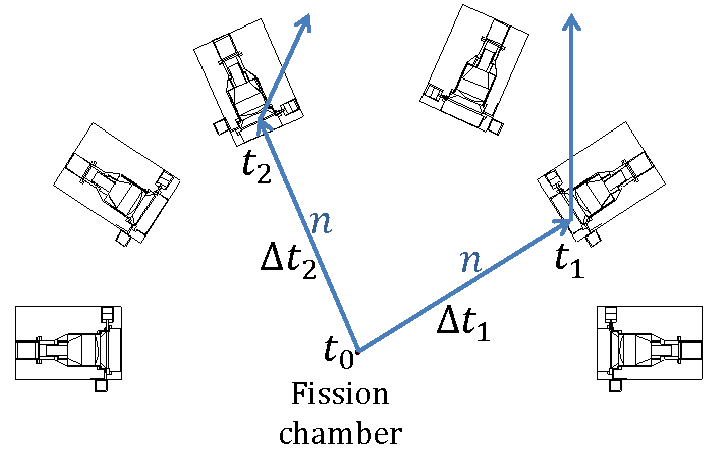
\includegraphics[width=0.5\linewidth]{bicorrelation_sketch.pdf}
	\caption{\coloronline Schematic of a true bicorrelation event in which two prompt fission neutrons are detected in coincidence with their originating fission. The schematic used is a two-dimensional view through an arc of the detector array in the \mcnpxpolimi model. }
	\label{fig:sketch}
\end{figure}

This work will study the characteristics of bicorrelation events with respect to the angle between the neutrons; this will be referred to as the bicorrelation angle and is approximated as the angle between the centers of each detector with respect to the fission chamber.

\subsection{The Bicorrelation Distribution}\label{sec:bicorrelation_distribution}

This analysis will make use of the bicorrelation distribution: a two-dimensional distribution of time of flight or energy for bicorrelation neutron events. The energies are calculated from the times of flight with the assumption that the neutron traveled directly from the fission chamber to the detector. Slight differences in the distances from the fission chamber to each detector are incorporated. \figfirst{fig:bicorr} shows the bicorrelation distributions for the experiment and \polimi simulations. These distributions show the number of counts at each $(\Dto,\Dtt)$ or $(\Eo,\Et)$ pixel, normalized by the number of detector pairs, the number of fission events, and the pixel size. 

\begin{figure}[!t]
	\centering
	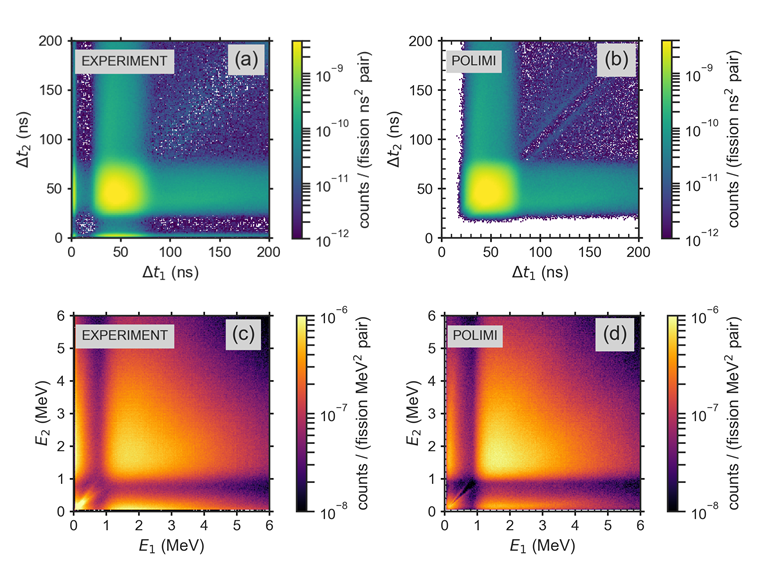
\includegraphics[trim={0cm 0cm 0cm 0cm},clip,width=7in]{bhm_all.png}
	\caption{\coloronline Bicorrelation time-of-flight distribution for (a) experimental data and (b) \polimi simulations, and bicorrelation energy distribution for (c) experimental data and (d) \polimi simulations.}
	\label{fig:bicorr}
\end{figure}

There are many interesting features in these distributions, a few of which are described here. The first observation is the primary feature produced by true prompt fission neutron bicorrelation events. In the time-of-flight distributions, this feature appears as a bright yellow spot within the approximate time window $25 < \Dti < \ns{75}$. In the energy distributions, this feature appears as a bright distribution extending to larger neutron energies from approximately $\Ei=\MeV{1}$ for each neutron, corresponding to the peak of the prompt fission neutron spectrum.

A second feature that can be observed in the bicorrelation distributions is the presence of accidental events, such as room return. In the time-of-flight distributions, these events appear at times beyond the true bicorrelation region, and dominate at $\Dti > \ns{75}$, where double-accidental events exist. Events in which a single accidental neutron is detected in coincidence with a true prompt fission neutron produce the wide bands emanating from the true bicorrelation region toward higher \Dti. When converted to neutron energy, these long time-of-flight events are mapped to very low energies and appear on the bicorrelation energy distribution as the bright yellow regions along the axes and as a bright spot at the origin. 

A third feature visible in the experiment time-of-flight distributions is PSD misclassification, which appears as the narrow bands along the $x$- and $y$-axes and as a localized spot at the origin. In this case, one or both of the particles is a gamma ray with a very small \Dti that has been misclassified as a neutron. While this feature in the time-of-flight distribution is very similar to the accidental event features in the energy distribution, they are, in fact, different. This feature due to misclassification does not appear in the \polimi distribution, as all simulations assume perfect PSD and thus do not include misclassified events. 

A final feature that is barely visible in these time-of-flight distributions is cross talk. This effect is explored in more detail in the next section. 

\subsection{Cross Talk}
Cross talk occurs when the same neutron interacts in multiple detectors and produces a false bicorrelation event. Cross talk is prevalent in detector pairs with small angular separation. Because full simulations were performed for all fission event generators, cross-talk events are present in all simulations and in the experimental data. %  are accidental bicorrelation events, and are not representative of true prompt fission bicorrelation neutrons. 
Although it is possible to remove cross talk on an average basis, as performed in~\refref{Marcath2016}, there is no way to remove cross talk on an event-by-event basis in experimental data. Therefore, cross-talk events and their effects on the bicorrelation analysis are present and will be discussed throughout this work.

Cross-talk events can be visually identified on small-angle bicorrelation distributions, as shown in \fig{fig:crosstalk} for a \polimi simulation of detector pairs at \degrees{15} and \degrees{45}. Cross-talk events appear as two diagonal bands in the bicorrelation time-of-flight and energy distributions. The line of cross talk can be defined as $\Dtt = \Dto + \Dtot$ when the neutron interacts first in detector 1, and \Dtot is the time-of-flight between detectors. Likewise, $\Dto = \Dtt + \Dtto$ describes the line of cross-talk events in which the neutron interacted first in detector 2. Then \Dtot will follow a distribution according to the energies of neutrons traveling from detector 1 to detector 2 and the distance between them. Thus, the $(\Dtt,\Dto)$ distribution will be diagonal lines with widths determined by the \Dtot distribution and offset from the identify line $\Dtt = \Dto$ by the magnitude of \Dtot. As the angle and distance between detectors increases, \Dtot increases and the cross-talk bands decrease in magnitude and departs farther from the identity line $\Dtt = \Dto$. The cross-talk features at long times ($>\ns{75}$) and low energies ($<\MeV{1}$) are largely due to accidental cross-talk events from room return or background. 

\begin{figure}[!t]
	\centering
	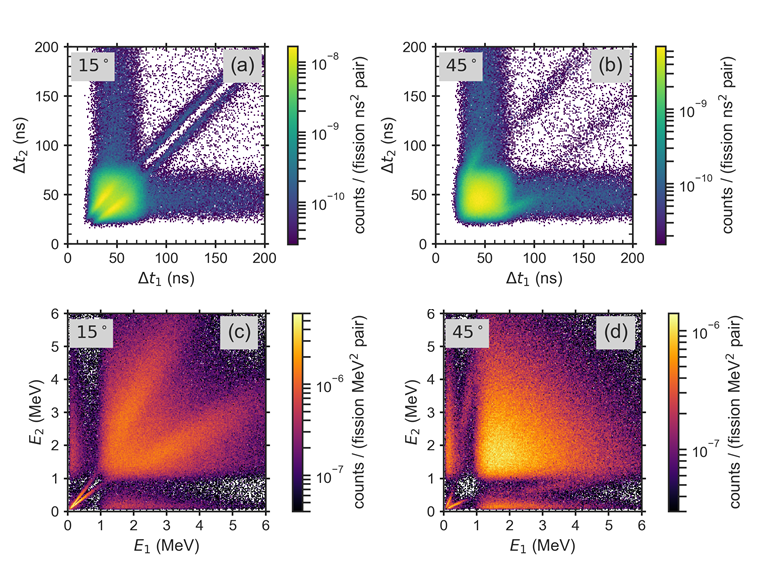
\includegraphics[trim={0cm 0.5cm .5cm .5cm},clip,width=7in]{bhm_ct.png}
	\caption{\coloronline Bicorrelation (a,b) time-of-flight and (c,d) energy distributions from \polimi simulation showing cross-talk effects, displayed for  detector pairs at (a,c) \degrees{15} and (b,d) \degrees{45}. The diagonal bands in each distribution include cross-talk events, which move farther from the identity line ($\Dto=\Dtt$ and $\Eo=\Et$) and decrease in magnitude as the angle between detectors increases. }
	\label{fig:crosstalk}
\end{figure}

Cross-talk effects are prominent at \degrees{15} and visible in some distributions up to \degrees{75}. Regions that may be affected by cross talk are displayed with gray background in the analysis plots in the next section. 

\section{Analysis and Results}

\subsection{Anisotropy in Neutron Emission Rate}\label{sec:asym}

Neutron emission from \Cftft spontaneous fission is assumed to occur after the fission fragments are in motion and traveling in opposite directions~\cite{Vorobyev2009}, assuming all neutrons are emitted from fully-accelerated fragments. Scission neutrons, emitted isotropically in the \Cftft rest frame and estimated to be $0-20\%$ of prompt neutron emission~\cite{Vogt2014,Petrov2005,Chietera2018}, are not included in the models or simulations discussed here.

In our simulations, we assume that neutron emission is isotropic in the rest frame of each fission fragment but anisotropic in the laboratory frame of motion. Thus, the direction of neutron emission follows that of the fission fragment that emitted it so that neutrons emitted in the direction of the fission fragment will receive an energy boost. The anisotropy can be characterized by calculating the count rate of bicorrelation events in detector pairs as a function of bicorrelation angle. The relative bicorrelation count rate, \Wij, for each pair of detectors $i$ and $j$, is defined as~\cite{Mueller2016}

\begin{equation}
\label{eq:Wij}
\Wij = \frac{\Dij}{\Si \Sj}
\end{equation}
where \Dij is the doubles count rate, and \Si and \Sj are the corresponding singles count rates. Each of these rates are determined from the number of counts in the energy range \MeV{1} to \MeV{4}. This conservative energy range was selected to minimize threshold effects at low energies and gamma-ray misclassification at higher energies while maximizing statistics. This analysis corrects for slight variations in efficiency between detectors.

An average \W was calculated for detector pairs in each \degrees{10}  bin, \Wtheta. \figfirst{fig:W}(a) shows \Wtheta for all four data sets, normalized by the integral over the distribution. The angle is plotted at the midpoint of the bins. For example, the data points at \degrees{15} include all pairs in the range $(\degrees{10},\degrees{20}]$. The error in \Wtheta was calculated as the standard deviation of \Wij values in that angular range, and is influenced by the variation in \W and the angular distribution in detector pair angles in that range. The error bar on the data point at \degrees{25}, for instance, is larger than most others, because the detector pairs in that bin are more evenly distributed across the represented angle range, as illustrated by the standard deviation in \fig{fig:det_df} and the slope of \Wtheta is high in that region. This error is larger than the propagated statistical error and attempts to incorporate systematic errors. 

\begin{figure}[!t]	
	\centering
	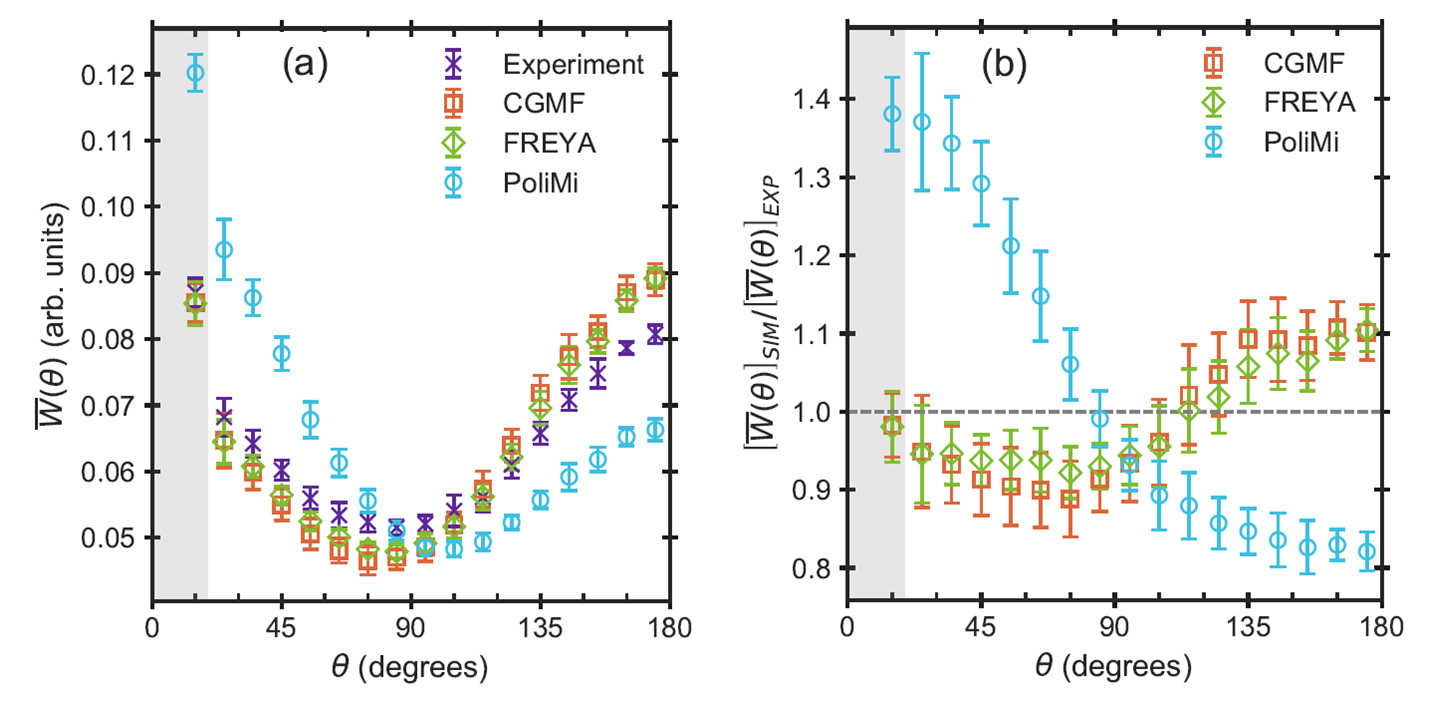
\includegraphics[trim={0cm 0cm 0cm 0cm},clip,width=7in]{W_figs.png}	
	\caption{\coloronline (a) Relative bicorrelation count rate \Wtheta for events from \MeV{1} to \MeV{4}, normalized by integral. (b) Ratio between relative bicorrelation rate for each simulation to that from experiment. The gray region from \degrees{0} to \degrees{20} serves as a reminder that cross talk is significant over this range.}
	\label{fig:W}
\end{figure}

All four datasets in \fig{fig:W}(a) produce smoothly-varying distributions with a local maximum at \degrees{15} where cross talk is prevalent, a minimum near \degrees{90}, and a local maximum at \degrees{175}. The minimum angle varies from \degrees{75} for \cgmf to \degrees{85} for \freya and the experiment to \degrees{105} in \polimi. The experimental result and the \polimi simulation agree within uncertainties with previous work with lower angular resolution~\cite{Larsen2014}. The largest magnitude of change between $\Wth{175}$ and $\Wth{85}$ is found with \cgmf, while the smallest magnitude of change is seen in \polimi. 

The most striking difference is that the \polimi result is tilted to the left, while the \cgmf, \freya, and experimental results are tilted to the right. The tilt of the angular correlation is strongly tied to the sharing of excitation energy between fission fragments. The complete event models \cgmf and \freya handle this sharing by giving some additional energy to the light fragment. In \freya, this is done with the $x$ parameter, defined as the advantage in excitation energy given to the light fragment~\cite{Vogt2014}, where $x$ is an adjustable input parameter expected to be larger than 1. The best fit value of $x$ for \freya with \Cftft(sf) was found to be 1.27~\cite{VanDyke2018}.  

In \cgmf, the energy sharing is done in a similar way except that the $x$ parameter is not a single value but is based on the ratio of neutron multiplicities of the light and heavy fragment pairs as a function of fragment mass, $R_T(A)$, to match the $\nu(A)$ data. When a single value of $R_T$ is used, the resulting $\nu(A)$ is similar to that of \freya with $x=1.27$~\cite{Talou2011}. 

A larger value of $x$ makes the distribution tilt toward \degrees{0} as the light fragment receives more energy and emits more neutrons, increasing the zero degree correlation. A value of $x$ near 1 makes the distribution tilt more strongly toward \degrees{180} as the energy is split more evenly between fragments. The \polimi result corresponds to $x\sim2$, giving the light fragment twice as much energy as the heavy fragment which is not physically realistic. This discrepancy is a side effect of how \polimi samples each quantity independently and does not capture effects related to the de-excitation process. 

\figfirst{fig:W}(b) shows \Wtheta from each simulation divided by that for experiment. This ratio shows that, compared to the measured results, \polimi overpredicts \Wtheta by up to 90\% at low angles and underpredicts at high angles, while \cgmf and \freya underpredict at low angles and overpredict at high angles by a much smaller amount, about 10\% in each case. This discrepancy may indicate that \cgmf and \freya predict too many two-neutron events in which one neutron comes from one fragment and the other neutron from the complementary fragment, as opposed to both neutrons coming from the same fragment. 

This variation can be explored further by capturing the magnitude of the anisotropy as a one-dimensional parameter \Asym
\begin{equation}
\label{eq:Asym}
\Asym = \frac{W(180)}{W(90)}\approx\frac{\Wth{175}}{\Wth{85}}.
\end{equation}
Due to the \degrees{10} wide discretization of angles, the data are compared at \degrees{175} and \degrees{85}, which include pairs at $(\degrees{170},\degrees{180}]$ and $(\degrees{80},\degrees{90}]$, respectively.

The anisotropy in neutron energy can be observed by varying the neutron energy threshold, as shown in \fig{fig:Asym_vs_Emin}. The magnitude of the anisotropy increases as the energy threshold is increased and lower energy neutrons are omitted from the analysis. This increase occurs because neutrons detected at angles near \degrees{180} are likely emitted from different fission fragments in their direction of travel and therefore receive a boost in energy due to the direction of motion. This boost also occurs for neutron pairs emitted at \degrees{0}, however, the Chi-Nu array cannot identify events at \degrees{0} where two neutrons interact in the same detector. 
Neutrons detected at angles near \degrees{90} did not receive this boost and therefore are emitted with lower energies. Thus, as the energy threshold is increased, events at angles near \degrees{90} are more likely to be removed from the population than events at \degrees{180}, thereby increasing \Asym. 

\figfirst{fig:Asym_vs_Emin}(a) shows that \cgmf consistently produces the highest values of \Asym while \polimi consistently produces the lowest.  Note also that the uncertainties grow as \Emin increases because there are fewer events in the population, limiting statistics. \figfirst{fig:Asym_vs_Emin}(b) shows the ratio of each of the simulations to the experimental data. This ratio is roughly independent of $\Emin$ at $\sim0.8$ for \polimi, while \cgmf and \freya vary slightly as \Emin increases. The \freya ratio starts at $\sim1.2$ and drops toward to 1 as \Emin increases, while the \cgmf ratio starts at 1.2 and grows larger with increasing \Emin.

\begin{figure}[!t]
	\centering
	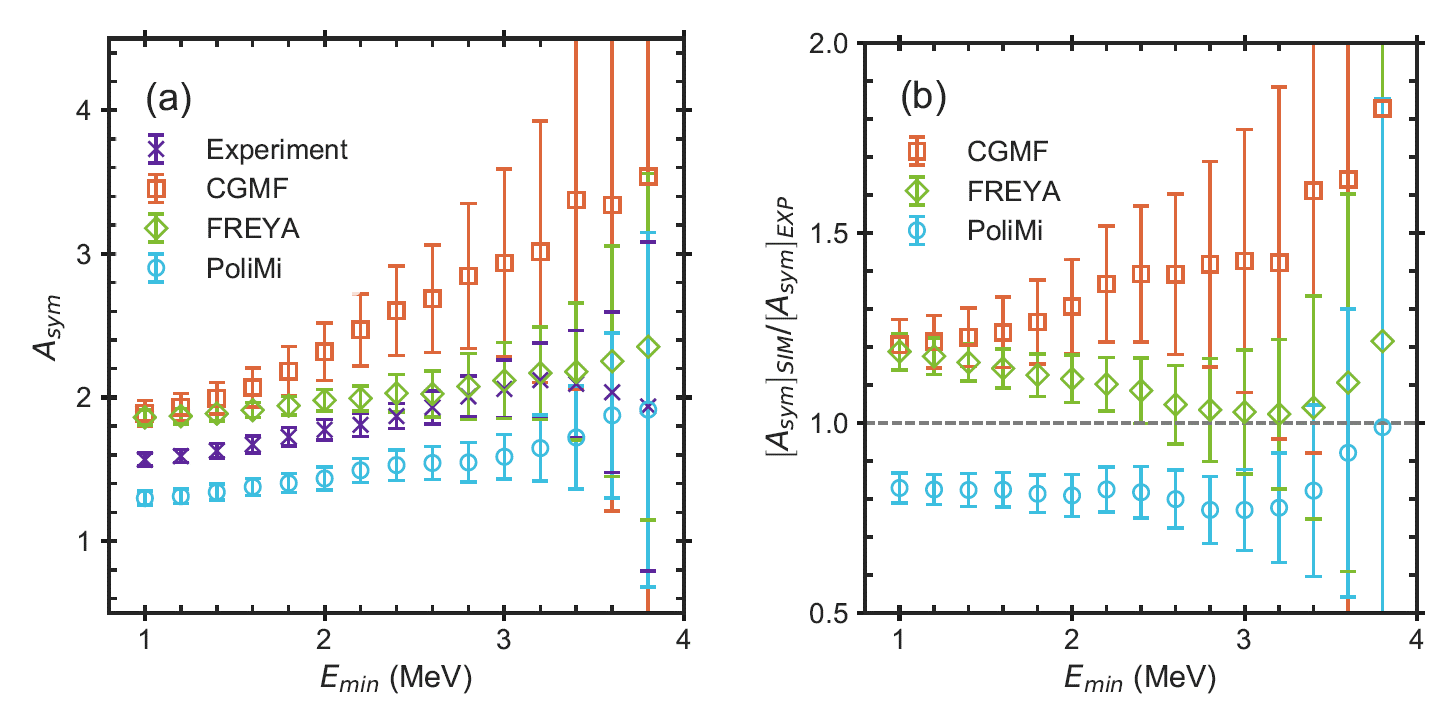
\includegraphics[trim={0cm 0cm 0cm 0cm},clip,width=7in]{Asym_figs.png}
	\caption{\coloronline (a) Magnitude of the neutron emission anisotropy, \Asym, as a function of \Emin and (b) ratio between simulated results and measured data. The magnitude of anisotropy increases as the neutron population is limited to higher energies. The error bars increase with \Emin as fewer events are included in the analysis, worsening statistics.}
	\label{fig:Asym_vs_Emin}
\end{figure}

\subsection{Neutron Energy Characteristics}

As stated in \secref{sec:asym}, the energies of prompt fission neutrons vary with their direction of emission relative to the direction of fission fragment motion. In detected bicorrelation events, this boost increases the average detected energies of pairs near \degrees{180}, which are likely to be emitted from opposite fragments in the fragment direction of motion. One can observe this effect by calculating the average neutron energy for neutrons in the 1~to~\MeV{4} range detected in bicorrelation events, defined as

\begin{equation}
\label{eq:Eave}
\Eave = \overline{(E_1+E_2)}/2.
\end{equation}
and shown as a function of bicorrelation angle in \fig{fig:Esum}(a). As stated in \secref{sec:asym}, this energy range is chosen to remove events at low energies that may have threshold effects and events at high energies that are gamma rays misclassified as neutrons. This average energy calculation does not provide a measurement of the average energy of the entire neutron population, but rather that in the 1~to~\MeV{4} range as a benchmark for comparison. This distribution shows that, in all cases, the average neutron energy reaches a minimum near \degrees{90} and increases steadily until it reaches a local maximum at \degrees{180}. Note that \Eave is higher than expected at \degrees{15} due to cross-talk effects; the gray band for angles less than \degrees{20} is a reminder of this. 

Although the shapes are approximately the same in all cases for angles less than \degrees{90}, the behavior varies greatly above \degrees{90}. First, the minimum \Eave for \cgmf occurs at \degrees{85} while for all other results it is at \degrees{95}. Second, \cgmf has the steepest increase in \Eave at angles up to \degrees{180}. Third, the experimental results are in excellent agreement with \freya at angles below \degrees{125}, but the value of \Eave for \freya levels out at higher angles while the \Eave of the data continues to rise. 

\figfirst{fig:Esum}(b) shows the ratio between each simulation and experiment, demonstrating that the agreement among all results is very good, as all simulations are within 3\% of the experimental data. \polimi produces consistently lower energies than experiment while \cgmf produces lower energies below \degrees{135} and higher energies above \degrees{135}. \freya agrees with experiment below \degrees{125}, but it produces lower average energies above this angle.

\begin{figure}[!t]	
	\centering
	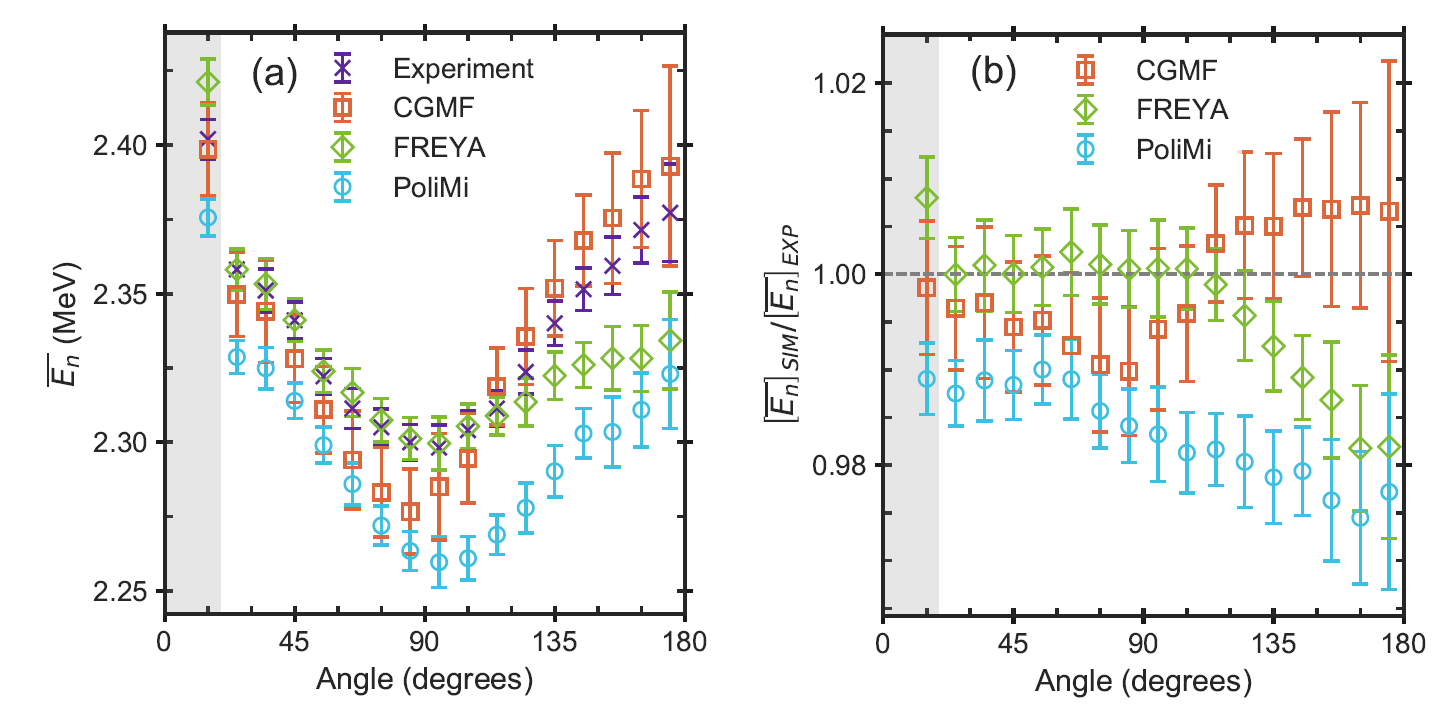
\includegraphics[trim={0cm 0cm 0cm 0cm},clip,width=7in]{Esum_figs.png}
	
	\caption{\coloronline (a) Average neutron energy as a function of bicorrelation angle across a range of \MeV{1} to \MeV{4}. (b) Ratio between average simulated energy and average measured energy, demonstrating agreement within 3\% across all data. The gray region from \degrees{0} to \degrees{20} serves as a reminder that cross talk is significant over this range.}
	\label{fig:Esum}
\end{figure}

While \fig{fig:Esum} provides a measurement of the energy distribution across the entire neutron population, it does not demonstrate whether the energy of one neutron depends on the energy of its bicorrelation partner. To determine this dependence, for fixed \Ei of \MeV{2} and \MeV{3}, the average energy \Ejave of the partner neutron is shown as a function of $\theta$ in \fig{fig:Ejave_vs_theta}. 

The distributions shown in \fig{fig:Ejave_vs_theta} share the same features as in \fig{fig:Esum}(a), although the behavior of data at angles less than \degrees{30} varies due to the effect of cross talk on \Ei. In fact, no significant angular dependence was observed in the shape of \Eave or \Ejave at any \Ei. 

\begin{figure}[!t]
	\centering	
	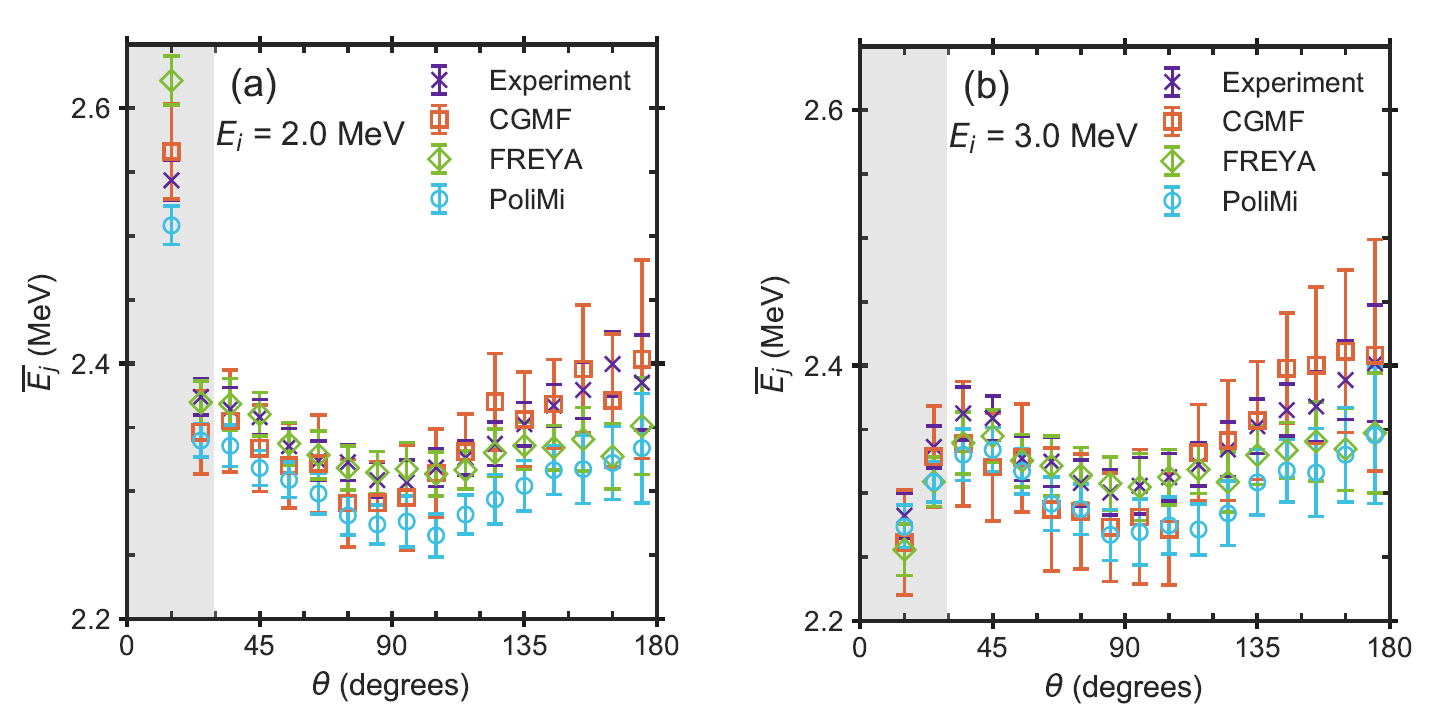
\includegraphics[trim={0cm 0cm 0cm 0cm},clip,width=7in]{Eave_at_2_3.png}
	\caption{\coloronline Average energy of neutrons across a range of \MeV{1} to \MeV{4} detected in coincidence with a (a) \MeV{2} and (b) \MeV{3} neutron.}
	\label{fig:Ejave_vs_theta}
\end{figure}

\begin{figure}[!t]
	\centering
	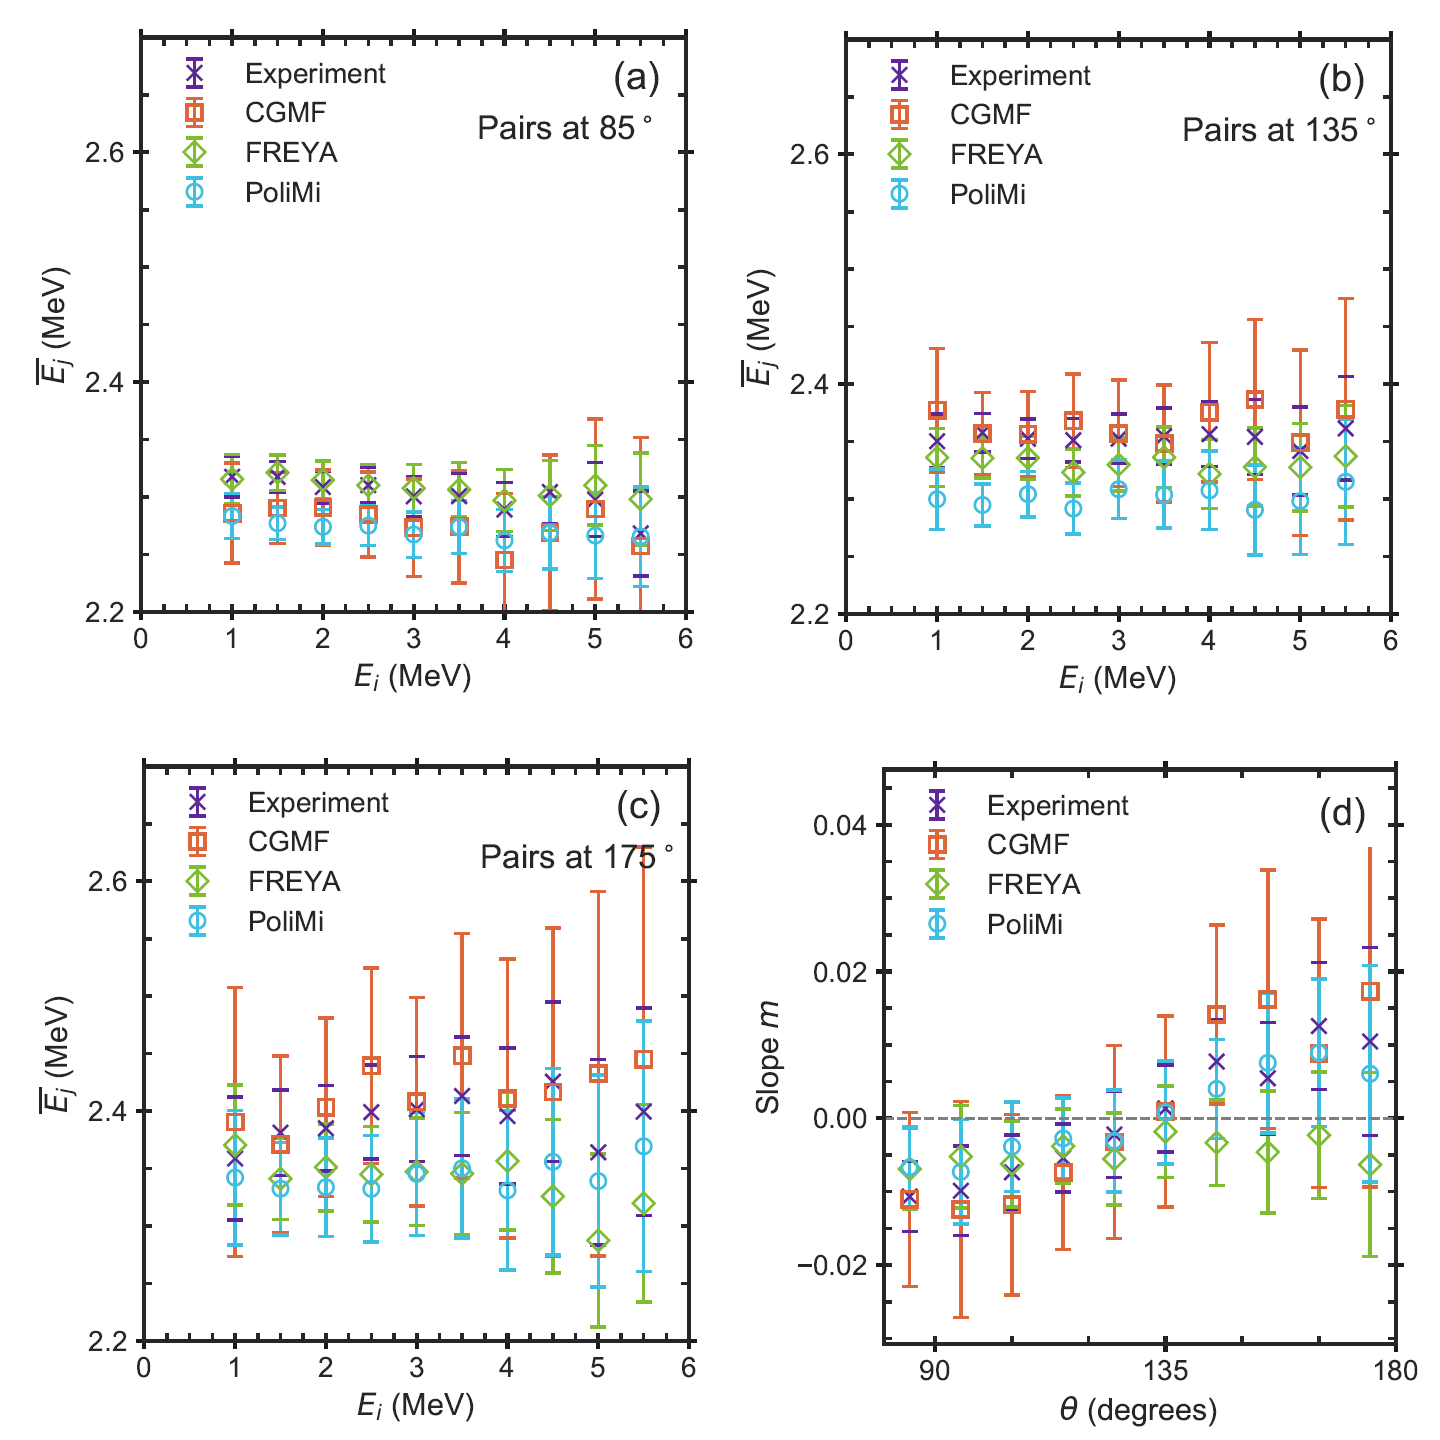
\includegraphics[trim={0cm 0cm 0cm 0cm},clip,width=7in]{E_slope.png}
	\caption{\coloronline Average correlated neutron energy \Ejave for fixed energy \Ei for detector pairs at (a) \degrees{85}, (b) \degrees{135}, and (c) \degrees{175}, and (d) slope of least-squares fit to $\Ejave(\Ei)$ at angles \degrees{85} and higher.} 
	\label{fig:Ejave_vs_Ei}
\end{figure}

Some differences were seen, however, in the values of \Ejave as \Ei is varied. The dependence of \Ejave on \Ei can be enhanced by studying \Ejave as a function of \Ei at a fixed bicorrelation angle, as shown in \fig{fig:Ejave_vs_Ei}. 
\figfirst{fig:Ejave_vs_Ei} (a)-(c) shows $\Ejave(\Ei)$ at bicorrelation angles \degrees{85}, \degrees{135}, and \degrees{175}. While it is not immediately clear to the naked eye whether a dependence of \Ejave on \Ei exists, one can perform a least-squares linear regression on the data and determine whether there is a statistically significant nonzero slope, $m$, as shown in \fig{fig:Ejave_vs_Ei}(d). Angles below \degrees{85} are omitted, because cross talk was shown to be significant enough to contaminate the calculation of the slope at lower angles.

The error bars in Figs.~\ref{fig:Esum},~\ref{fig:Ejave_vs_theta}, and~\ref{fig:Ejave_vs_Ei} vary firstly with sample size and are smaller in angle bins with more detector pairs. Error bars are largest in the two highest angle bins, which have the lowest number of detector pairs, as shown in \fig{fig:det_df}.

There are several interesting aspects of this distribution. First and foremost, all four results have slopes within $2\sigma$ of $m=0.0$ across all angles. Thus, there is no statistically significant slope in any of the datasets. However, trends do exist in the data which will be discussed here and will be the subject of future work in order to reduce uncertainties and determine whether the trends are significant. 


All results, data and simulations, show a negative slope near \degrees{90}. Above \degrees{140}, the slope of the data, as well as that of the \cgmf and \polimi simulations, becomes positive, crossing zero near \degrees{135}. Since events with bicorrelation angle near \degrees{90} are likely emitted from the same fragment, the negative slope at angles near \degrees{90} could indicate that neutrons emitted from the same fission fragment compete with one another for energy. Events with neutrons emitted near \degrees{180} are likely to come from different fission fragments, indicating that there may be some positive correlation in neutron energies emitted from different fission fragments. Note that, the \freya simulation results in negative slope across all angles, indicating that correlated neutrons produced by \freya may compete with one another for energy regardless of whether or not they were produced by the same fission fragment. 

\section{Conclusion}

This work investigated correlations in angle and energy between prompt neutrons emitted in the same \Cftft spontaneous fission event, including measuring the energy dependence between correlated neutrons for the first time. Experiments were performed using 42 components of the Chi-Nu detector array in a hemispherical configuration surrounding a fission chamber. The detector array was simulated in \mcnpxpolimi with three different fission models: \polimiipol, \cgmf, and \freya.

Characteristics of the correlated neutrons were studied with respect to the angle between the two neutrons. The large number of detectors produced a broad distribution of bicorrelation angles collected into \degrees{10} bins. The \meters{1} flight path allowed for experimental timing resolution as low as \ns{1}, allowing excellent energy resolution to be attained for neutron energies between \MeV{1} and \MeV{4} from the time-of-flight calculations. 

The simulations showed good agreement with experiment for all measured quantities, while revealing interesting differences between fission event generators. The neutron emission anisotropy generated by \cgmf and \freya agreed within 10\% of experiment, while underpredicting the anisotropy at small angles and overpredicting it at high angles. On the other hand, \polimi showed poor agreement, differing up to 40\% from experiment at low angles. All simulated average neutron energies fell within 3\% of the experimental data. \freya produced the best agreement with experiment: the average neutron energies agreed with the data to 0.5\% for angles below \degrees{135}.

The average neutron energy was found to be negatively correlated with the energy of its correlated partner for pairs at \degrees{85}, indicating that neutrons may compete for emission energy at low angles, where neutrons are likely to be emitted from the same fission fragment. This correlation was found to be positive for pairs at \degrees{175}, where neutrons are likely to be emitted from different fission fragments. However, this result is inconclusive because the uncertainties in the measurements result in  calculated slopes within $2\sigma$ of 0. Further experiments should be performed to study this effect in greater detail. 

These conclusions lead to further questions that could be pursued by more sophisticated experiments. The ability to distinguish events with neutrons from the same fission fragment would determine whether there is a competition for energy within the energy spectrum of the fragment, such as a reduction in the average emission energy for each subsequent neutron emission. Tracking the fission fragments would allow this analysis to be repeated with respect to the fission fragment motion. Additionally, that would also enable experimental measurement of differences due to energy sharing between fragments of $\nu(A)$, $\epsilon(A)$ (where $\epsilon$ is the average neutron kinetic energy), $\nu(\text{TKE})$, and neutron-light fragment correlations, specifically for a given $A_L$. A comparison of these results are shown from \freya and \cgmf in \refref{Talou2018}. Extracting information about the neutrons at the time of their emission from the fragments, as opposed to relying on the information gleaned from the neutrons arriving at the detectors, which may have undergone some rescattering, would enable more direct comparison to the complete fission event models. Finally, repeating this measurement with \Putf(sf), with an average neutron multiplicity closer to 2 $(\sim2.15)$ than \Cftft(sf) $(\overline \nu \sim3.76)$, would reduce the number of fission events with multiple neutron pairs in the same event. Thus, in this case, detected bicorrelation events are more likely to come from events where exactly two neutrons are emitted: either one from each fragment or two from the same fragment.

\section*{Acknowledgments}

This work was performed under the auspices of the U.S. Department of Energy by Los Alamos National Security, LLC, under Contract No.~DE-AC52-06NA25396, by Lawrence Livermore National Security, LLC under Contract No.~DE-AC52-07NA27344, by Lawrence Berkeley National Laboratory under Contract DE-AC02-05CH11231, by the Consortium for Verification Technology under Contract No.~DE-NA0002534, by the Office of Nuclear Physics in the Office of Science under Contract No.~DE-AC02-05CH11231, and by the University of Michigan.


%%%%%%%%%%%%%% START BACKUP INFORMATION / APPENDICES %%%%%%%%%%%%%%%%
%% References with bibTeX database:
\bibliographystyle{elsarticle-num}
% For the revisions, I am just going to modify the formatted citations below and NOT use the .bib file.

\begin{thebibliography}{10}
	\expandafter\ifx\csname url\endcsname\relax
	\def\url#1{\texttt{#1}}\fi
	\expandafter\ifx\csname urlprefix\endcsname\relax\def\urlprefix{URL }\fi
	\expandafter\ifx\csname href\endcsname\relax
	\def\href#1#2{#2} \def\path#1{#1}\fi
	
	\bibitem{Fraser1952a}
	J.~S. Fraser, {The angular distribution of prompt neutrons emitted in fission},
	Physical Review 88~(3) (1952) 536--541.
	\newblock \href {https://doi.org/10.1103/PhysRev.88.536}
	{\path{doi:10.1103/PhysRev.88.536}}.
	
	\bibitem{Skarsvag1970}
	K.~Skarsvag, {Time distribution of gamma-rays from spontaneous fission of
		Cf-252}, Nuclear Physics A 153 (1970) 82--96.
	\newblock \href {https://linkinghub.elsevier.com/retrieve/pii/0375947470907578}
	{\path{doi:10.1016/0375-9474(70)90757-8}}.
	
	\bibitem{Bowman1962}
	H.~R. Bowman, S.~G. Thompson, J.~C.~D. Milton, W.~J. Swiatecki, {Velocity and
		angular distributions of prompt neutrons from spontaneous fission of Cf252},
	Physical Review 126~(6) (1962) 2120--2136.
	\newblock \href {https://doi.org/10.1103/PhysRev.126.2120}
	{\path{doi:10.1103/PhysRev.126.2120}}.
	
	\bibitem{Larsen2014}
	S.~Pozzi, B.~Wieger, A.~Enqvist, S.~Clarke, M.~Flaska, M.~Marcath, E.~Larsen,
	R.~Haight, E.~Padovani, {Correlated Neutron Emissions from 252Cf}, Nuclear
	Science and Engineering 178~(2) (2014) 250--260.
	\newblock \href {https://doi.org/10.13182/NSE13-96}
	{\path{doi:10.13182/NSE13-96}}.
	
	\bibitem{Pozzi2012}
	S.~Pozzi, S.~Clarke, W.~Walsh, E.~Miller, J.~Dolan, M.~Flaska, B.~Wieger,
	A.~Enqvist, E.~Padovani, J.~Mattingly, D.~Chichester, P.~Peerani,
	{MCNPX-PoliMi for nuclear nonproliferation applications}, Nuclear Instruments
	and Methods in Physics Research Section A: Accelerators, Spectrometers,
	Detectors and Associated Equipment 694 (2012) 119--125.
	\newblock \href {https://doi.org/10.1016/J.NIMA.2012.07.040}
	{\path{doi:10.1016/J.NIMA.2012.07.040}}.
	
	\bibitem{Talou2013}
	P.~Talou, T.~Kawano, I.~Stetcu, {Prompt Fission Neutrons and Gamma Rays in a
		Monte Carlo Hauser-Feshbach Formalism}, Physics Procedia 47 (2013) 39--46.
	\newblock \href {https://doi.org/10.1016/J.PHPRO.2013.06.007}
	{\path{doi:10.1016/J.PHPRO.2013.06.007}}.
	
	\bibitem{Talou2014}
	P.~Talou, I.~Stetcu, T.~Kawano, {Modeling the Emission of Prompt Fission
		$\gamma$ Rays for Fundamental Physics and Applications}, Physics Procedia 59
	(2014) 83--88.
	\newblock \href {https://doi.org/10.1016/J.PHPRO.2014.10.013}
	{\path{doi:10.1016/J.PHPRO.2014.10.013}}.
	
	\bibitem{Talou2016}
	P.~Talou, T.~Kawano, I.~Stetcu, J.~P. Lestone, E.~McKigney, M.~B. Chadwick,
	{Late-time emission of prompt fission $\gamma$ rays}, Physical Review C
	94~(6) (2016) 064613.
	\newblock \href {https://doi.org/10.1103/PhysRevC.94.064613}
	{\path{doi:10.1103/PhysRevC.94.064613}}.
	
	\bibitem{Randrup2009}
	J.~Randrup, R.~Vogt, {Calculation of fission observables through event-by-event
		simulation}, Physical Review C 80~(2) (2009) 024601.
	\newblock \href {https://doi.org/10.1103/PhysRevC.80.024601}
	{\path{doi:10.1103/PhysRevC.80.024601}}.
	
	\bibitem{Vogt2011}
	R.~Vogt, J.~Randrup, {Event-by-event study of neutron observables in
		spontaneous and thermal fission}, Physical Review C 84~(4) (2011) 044621.
	\newblock \href {https://doi.org/10.1103/PhysRevC.84.044621}
	{\path{doi:10.1103/PhysRevC.84.044621}}.
	
	\bibitem{Vogt2013}
	R.~Vogt, J.~Randrup, {Event-by-event study of photon observables in spontaneous
		and thermal fission}, Physical Review C 87~(4) (2013) 044602.
	\newblock \href {https://doi.org/10.1103/PhysRevC.87.044602}
	{\path{doi:10.1103/PhysRevC.87.044602}}.
	
	\bibitem{Vogt2014}
	R.~Vogt, J.~Randrup, {Neutron angular correlations in spontaneous and
		neutron-induced fission}, Physical Review C 90~(6) (2014) 064623.
	\newblock \href {https://doi.org/10.1103/PhysRevC.90.064623}
	{\path{doi:10.1103/PhysRevC.90.064623}}.
	
	\bibitem{Randrup2014}
	J.~Randrup, R.~Vogt, {Refined treatment of angular momentum in the
		event-by-event fission model freya}, Physical Review C 89~(4) (2014) 044601.
	\newblock \href {https://doi.org/10.1103/PhysRevC.89.044601}
	{\path{doi:10.1103/PhysRevC.89.044601}}.
	
	\bibitem{Vogt2017}
	R.~Vogt, J.~Randrup, {Improved modeling of photon observables with the
		event-by-event fission model freya}, Physical Review C 96~(6) (2017) 064620.
	\newblock \href {https://doi.org/10.1103/PhysRevC.96.064620}
	{\path{doi:10.1103/PhysRevC.96.064620}}.
	
	\bibitem{Verbeke2018}
	J.~Verbeke, J.~Randrup, R.~Vogt, {Fission Reaction Event Yield Algorithm FREYA
		2.0.2}, Computer Physics Communications 222 (2018) 263--266.
	\newblock \href {https://doi.org/10.1016/J.CPC.2017.09.006}
	{\path{doi:10.1016/J.CPC.2017.09.006}}.
	
	\bibitem{Miller2012}
	E.~C. Miller, S.~D. Clarke, M.~Flaska, S.~A. Pozzi, E.~Padovani, {Journal of
		nuclear materials management.}, Vol.~40, Institute of Nuclear Materials
	Management, 2012.
	
	\bibitem{Talou2018}
	P.~Talou, \etal. {Correlated Prompt Fission Data in Transport Simulations,} Eur. Phys. J. A54 (2018) No.~1, 9. \newblock \href {http://inspirehep.net/record/1628151} {\path{doi:10.1140/epja/i2018-12455-0}}.
	
	\bibitem{Frame2007}
	K.~Frame, W.~Clay, T.~Elmont, E.-I. Esch, P.~Karpius, D.~MacArthur,
	E.~McKigney, P.~Santi, M.~Smith, J.~Thron, R.~Williams, {Development of a
		liquid scintillator neutron multiplicity counter (LSMC)}, Nuclear Instruments
	and Methods in Physics Research Section A: Accelerators, Spectrometers,
	Detectors and Associated Equipment 579~(1) (2007) 192--195.
	\newblock \href {https://doi.org/10.1016/j.nima.2007.04.038}
	{\path{doi:10.1016/j.nima.2007.04.038}}.
	
	\bibitem{DiFulvio2017}
	A.~{Di Fulvio}, T.~Shin, T.~Jordan, C.~Sosa, M.~Ruch, S.~Clarke, D.~Chichester,
	S.~Pozzi, {Passive assay of plutonium metal plates using a fast-neutron
		multiplicity counter}, Nuclear Instruments and Methods in Physics Research
	Section A: Accelerators, Spectrometers, Detectors and Associated Equipment
	855 (2017) 92--101.
	\newblock \href {https://doi.org/10.1016/j.nima.2017.02.082}
	{\path{doi:10.1016/j.nima.2017.02.082}}.
	
	\bibitem{Mueller2016}
	J.~M. Mueller, J.~Mattingly, {Using anisotropies in prompt fission neutron
		coincidences to assess the neutron multiplication of highly multiplying
		subcritical plutonium assemblies}, Nuclear Instruments and Methods in Physics
	Research, Section A: Accelerators, Spectrometers, Detectors and Associated
	Equipment 825 (2016) 87--92.
	\newblock \href {https://doi.org/10.1016/j.nima.2016.04.027}
	{\path{doi:10.1016/j.nima.2016.04.027}}.
	
	\bibitem{Holewa2013}
	L.~Holewa, W.~Charlton, E.~Miller, S.~Pozzi, {Using neutron angular anisotropy
		information to dynamically determine the ratio of the (alpha,n) rate to
		spontaneous fission rate for coincidence counting applications}, Nuclear
	Instruments and Methods in Physics Research, Section A: Accelerators,
	Spectrometers, Detectors and Associated Equipment 701 (2013) 249--253.
	\newblock \href {https://doi.org/10.1016/j.nima.2012.11.026}
	{\path{doi:10.1016/j.nima.2012.11.026}}.
	
	\bibitem{Perdue2014}
	B.~Perdue, T.~Taddeucci, R.~Haight, T.~Bredeweg, M.~Devlin, N.~Fotiades,
	M.~Jandel, A.~Laptev, H.~Lee, R.~Nelson, J.~O'Donnell, J.~Ullmann, S.~Wender,
	C.~Wu, E.~Kwan, A.~Chyzh, R.~Henderson, J.~Gostic, {Development of an Array
		of Liquid Scintillators to Measure the Prompt Fission Neutron Spectrum at
		LANSCE}, Nuclear Data Sheets 119 (2014) 371--372.
	\newblock \href {https://doi.org/10.1016/j.nds.2014.08.102}
	{\path{doi:10.1016/j.nds.2014.08.102}}.
	
	\bibitem{MarcathThesis2018}
	M.~J.~Marcath, (2018). Measured and Simulated Prompt Fission Neutron and Photon Correlations. University of Michigan. Retrieved from \newblock \href {https://deepblue.lib.umich.edu/handle/2027.42/147560} {\path{https://deepblue.lib.umich.edu/handle/2027.42/147560}}
	
	\bibitem{Verbeke2018b}
	J.~M. Verbeke, L.~F. Nakae, R.~Vogt, {Neutron-neutron angular correlations in
		spontaneous fission of Cf252 and Pu240}, Physical Review C 97~(4) (2018)
	044601.
	\newblock \href {https://doi.org/10.1103/PhysRevC.97.044601}
	{\path{doi:10.1103/PhysRevC.97.044601}}.
	
	\bibitem{Marcath2018}
	M.~J. Marcath, R.~C. Haight, R.~Vogt, M.~Devlin, P.~Talou, I.~Stetcu,
	J.~Randrup, P.~F. Schuster, S.~D. Clarke, S.~A. Pozzi, {Measured and
		simulated 252Cf(sf) prompt neutron-photon competition}, Physical Review C
	97~(4) (2018) 1--15.
	\newblock \href {https://doi.org/10.1103/PhysRevC.97.044622}
	{\path{doi:10.1103/PhysRevC.97.044622}}.
	
	\bibitem{Polack2015}
	J.~Polack, M.~Flaska, A.~Enqvist, C.~Sosa, C.~Lawrence, S.~Pozzi, {An algorithm
		for charge-integration, pulse-shape discrimination and estimation of
		neutron/photon misclassification in organic scintillators}, Nuclear
	Instruments and Methods in Physics Research Section A: Accelerators,
	Spectrometers, Detectors and Associated Equipment 795 (2015) 253--267.
	\newblock \href {https://doi.org/10.1016/j.nima.2015.05.048}
	{\path{doi:10.1016/j.nima.2015.05.048}}.
	
	\bibitem{Mattingly1998}
	J.~Mattingly, {High Order Statistical Signatures from Source-Driven
		Measurements of Subcritical Fissile Systems}, Ph.D. thesis, The University of
	Tennessee, Knoxville (1998).
	
	\bibitem{Marcath2016}
	M.~Marcath, T.~Shin, S.~Clarke, P.~Peerani, S.~Pozzi, {Neutron angular
		distribution in plutonium-240 spontaneous fission}, Nuclear Instruments and
	Methods in Physics Research, Section A: Accelerators, Spectrometers,
	Detectors and Associated Equipment 830 (2016) 163--169.
	\newblock \href {https://doi.org/10.1016/j.nima.2016.05.064}
	{\path{doi:10.1016/j.nima.2016.05.064}}.
	
	\bibitem{Vorobyev2009}
	A.~Vorobyev, O.~Shcherbakov, Y.~Pleva, A.~Gagarski, G.~Val'ski, G.~Petrov,
	V.~Petrova, T.~Zavarukhina, {Measurements of angular and energy distributions
		of prompt neutrons from thermal neutron-induced fission}, Nuclear Instruments
	and Methods in Physics Research Section A: Accelerators, Spectrometers,
	Detectors and Associated Equipment 598~(3) (2009) 795--801.
	\newblock \href {https://doi.org/10.1016/j.nima.2008.10.017}
	{\path{doi:10.1016/j.nima.2008.10.017}}.
	
	\bibitem{Oberer2000}
	R.~B.~Oberer, Maximum Alpha To Minimum Fission Pulse Amplitude for a Parallel-Plate and Hemispherical Cf-252 Ion-Chamber Instrumented Neutron Source, Oak Ridge National Laboratory Technical Report No. ORNL/TM-2000/290, 2000 (unpublished).	
	
	
	\bibitem{Petrov2005}
	G.~A. Petrov, H.~Goutte, H.~Faust, G.~Fioni, D.~Goutte, {Current status of the
		search for scission neutrons in fission and estimation of their main
		characteristics}, AIP Conference Proceedings 798 (2005) 205--212.
	\newblock \href {https://doi.org/10.1063/1.2137248}
	{\path{doi:10.1063/1.2137248}}.
	
	\bibitem{Chietera2018}
	A.~Chietera, L.~Stuttg{\'{e}}, F.~G{\"{o}}nnenwein, Y.~Kopatch, M.~Mutterer,
	A.~Gagarski, I.~Guseva, E.~Chernysheva, F.~J. Hambsch, F.~Hanappe,
	Z.~Mezentseva, S.~Telezhnikov, {Angular correlations in the prompt neutron
		emission of spontaneous fission of 252Cf}, The European Physical Journal A
	54~(6) (2018) 98.
	\newblock \href {https://doi.org/10.1140/epja/i2018-12529-y}
	{\path{doi:10.1140/epja/i2018-12529-y}}.
	
	\bibitem{VanDyke2018}
	J.~{Van Dyke}, L.~Bernstein, R.~Vogt, {Parameter Optimization and Uncertainty
		Analysis of FREYA for Spontaneous Fission} (2018) 1--13. \href
	{http://arxiv.org/abs/1809.05587} {\path{arXiv:1809.05587}}.
	
	\bibitem{Talou2011}
	P.~Talou, B.~Becker, T.~Kawano, M.~B.~Chadwick, Y.~Danon, {Advanced Monte Carlo modeling of prompt fission neutrons for thermal and fast neutron-induced fission reactions on 239Pu}, Physical Review C 83, 064612 (2011). \newblock \href{https://journals.aps.org/prc/abstract/10.1103/PhysRevC.83.064612} {\path{doi:10.1103/PhysRevC.83.064612}}
	
\end{thebibliography}


\end{document}